\documentclass[usenames,dvipsnames,mathserif,compress]{beamer}
\usepackage[utf8]{inputenc}
\usepackage[T1]{fontenc}
\usepackage{amsmath}
\usepackage{amssymb}
\usepackage{listings}

\lstset{%,
  basicstyle=\small\ttfamily,
  keywordstyle=\color{red},
  identifierstyle=\color{Blue},
  stringstyle=\color{yellow},
  showstringspaces=false,
  language=C}%,


\author{Ask Hjorth Larsen}

\begin{document}
\title{Introduction to high-performance computing}
%  hello world

\begin{frame}
  \maketitle
\end{frame}

\begin{frame}
  \frametitle{Floating point numbers}
  Computational physics mostly boils down to multiplying floating point numbers.
  \begin{block}{IEEE 754 standard for floating point numbers}
    \begin{itemize}
    \item Number is represented as $M \times 2^n$
    \item $M$ is the significand or mantissa
    \item $n$ is the exponent
    \end{itemize}
  \end{block}
  \begin{block}{Important types}
    \begin{itemize}
    \item 32-bit single precision: 24 bit for $M$, 8 for $n$
    \item 64-bit double precision: 53 bit for $M$, 11 for $n$
    \end{itemize}
  \end{block}
\end{frame}


\begin{frame}
  \frametitle{Pipelining}
  \begin{itemize}
  \item In one cycle, perform multiple operations on different data
  \item Pipelining
    \begin{tabular}{c|cccccccccccc}
      & u1 &u2&u3&u4&u5&u6&u7&\\\hline
      Cycle 1 & A &ø&ø&ø&ø&ø&ø& \\
      Cycle 2 & B & A &ø&ø&ø&ø&ø& \\
      Cycle 3 & C & B & A &ø&ø&ø&ø& \\
      Cycle 4 & D & C & B & A &ø&ø&ø& \\
      Cycle 5 & E & D & C & B & A &ø&ø& \\
      Cycle 6 & ø & E & D & C & B & A &ø& \\
      Cycle 7 & ø & ø & E & D & C & B & A \\
      Cycle 8 & ø & ø & ø & E & D & C & B \\
      Cycle 9 & ø & ø & ø & ø & E & D & C \\
      Cycle 10 &ø & ø & ø & ø & ø & E & D \\
    \end{tabular}
  \end{itemize}
\end{frame}

\begin{frame}
  \frametitle{Branching}
  \begin{itemize}
  \item We know that jumping around in memory when retrieving data is bad
  \item Jumping around in the \emph{code} is also bad as it breaks pipelining
  \item Branching constructes are: \texttt{if} statements, function calls, \texttt{goto}, \ldots
  \item Avoid branching as much as possible, particularly in inner loops
  \end{itemize}
\end{frame}


\begin{frame}
  \frametitle{Memory and multilevel caching}
  Example: Intel i7-4770 Haswell architecture\\
  \medskip
  \begin{tabular}{llll}
     & Size & Latency & Total \\
    \hline\hline
    L1 cache & 64 KB/core & 4--5 cycles & 1.3 ns\\
    L2 cache & 256 KB/core & 12 cycles & 3.5 ns \\
    L3 cache & 8 MB, shared & 36 cycles & 11 ns\\
    Main memory & 32 GB, shared & $36\textsf{ cycles} + 57$ ns & 68 ns\\\hline\hline
  \end{tabular}
  Source: \url{http://www.7-cpu.com/cpu/Haswell.html}
  %\medskip
  \begin{itemize}
  \item When accessing memory, contiguous chunks of memory will be copied into cache
  \item Cached memory access is very efficient
  \item A failed cache lookup is called a ``cache miss''
  \item Upon cache miss, element is looked up at next (slower) level
  \end{itemize}

\end{frame}



\begin{frame}
  \frametitle{Arrays and memory layout}
  \begin{itemize}
  \item  Standard mathematical matrix notation:
  \begin{align}
    \left[
  \begin{matrix}
    1,1 & 1,2 & 1,3 \\
    2,1 & 2,2 & 2,3 \\
    3,1 & 3,2 & 3,3
  \end{matrix}
  \right]
  \end{align}
\item Elements of the array are stored in a \alert{contiguous} chunk of memory,
  but the ordering depends on language
\item Fortran memory order is \alert{column-major}:
  \begin{tabular}{|c|c|c|c|c|c|c|c|c|}
    \hline
     $1,1$&$2,1$&$3,1$&$1,2$&$2,2$&$3,2$&$1,3$&$2,3$&$3,3$ \\\hline
  \end{tabular}
\item C memory order is \alert{row-major}:
  \begin{tabular}{|c|c|c|c|c|c|c|c|c|}
    \hline
     $1,1$&$1,2$&$1,3$&$2,1$&$2,2$&$2,3$&$3,1$&$3,2$&$3,3$ \\\hline
  \end{tabular}
\item Accessing elements in memory order is fast.
  \end{itemize}
\end{frame}

\begin{frame}[fragile]
  \frametitle{Optimizing cache use}
  \begin{itemize}
  \item Work on contiguous chunks of memory
  \end{itemize}
\begin{lstlisting}
for(i=0; i < N; i++) {
  for(j=0; j < M; j++) {
    a[i * N + j] = ...
  }
}
\end{lstlisting}
vs
\begin{lstlisting}
for(j=0; j < M; j++) {
  for(i=0; i < N; i++) {
    a[i * N + j] = ...
  }
}
\end{lstlisting}
\end{frame}

\begin{frame}[fragile]
  \frametitle{Benchmark}
  \begin{align}
    \hspace{-2cm} \textrm{Matrix multiplication}\quad c_{ij} &= \sum_k a_{ik} b_{kj}\nonumber
  \end{align}
\begin{lstlisting}
void matmul_ikj(int I, int J, int K,
                double *A, double *B, double *C)
{
  int i, j, k;
  for(i=0; i < I; i++) {
    for(k=0; k < K; k++) {
      for(j=0; j < J; j++) {
        C[i * J + j] += A[i * K + k] * B[k * J + j];
      }
    }
  }
}
\end{lstlisting}
Different permutations of $\{ikj\}$ loops will perform differently
\end{frame}


\begin{frame}
  \begin{figure}
  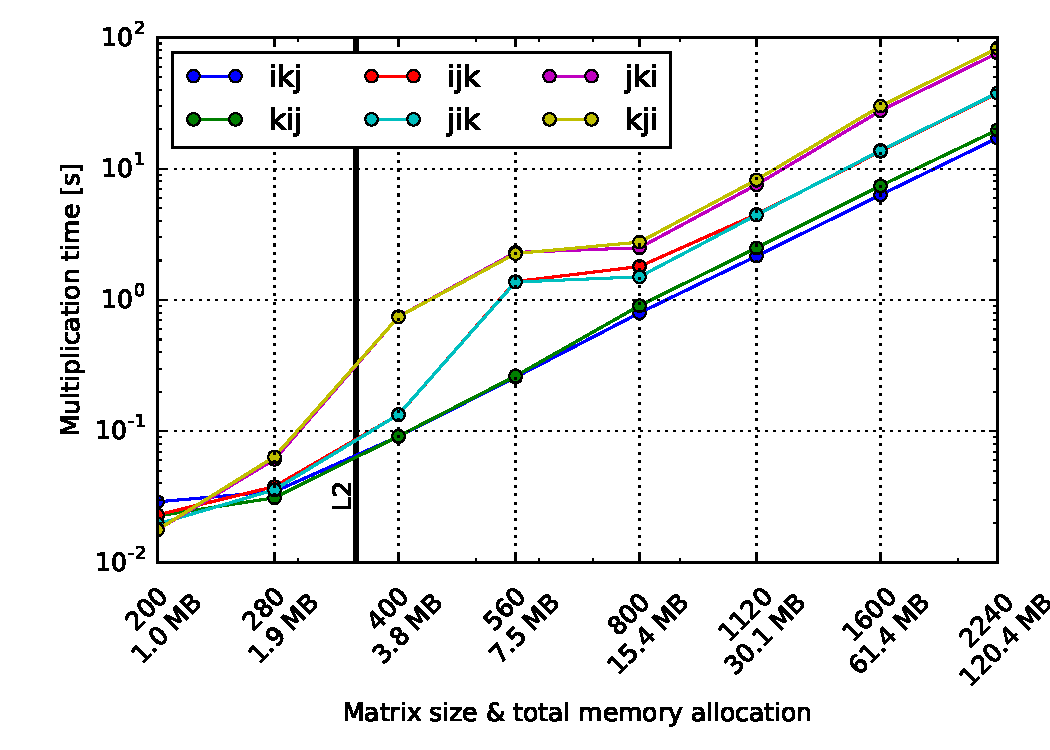
\includegraphics[width=\textwidth]{code/timings-matmul}
  \caption{Timings for matrix multiplication with different loop order}
  \end{figure}
\end{frame}

% Part 1: HPC
%  * floating point operations
%  * pipelining
%  * cache levels
%  * loop unrolling
%  * matmul
%  * BLAS

\begin{frame}[fragile]
  \frametitle{Loop unrolling}
\begin{lstlisting}
for(i=0; i < 4; i++) {
    a[i] = b[i] * c[i];
}
\end{lstlisting}
vs
\begin{lstlisting}
  a[i] = b[i] * c[i];
  a[i + 1] = b[i + 1] * c[i + 1];
  a[i + 2] = b[i + 2] * c[i + 2];
  a[i + 3] = b[i + 3] * c[i + 3];
\end{lstlisting}
\begin{itemize}
\item Eliminates bounds check on \texttt{i}
\item Compiler may be able to unroll automatically.
\end{itemize}
\end{frame}

\begin{frame}
  \frametitle{BLAS}
  \framesubtitle{Basic Linear Algebra Subroutines}
  \begin{itemize}
  \item Standard interface for standard operations:
    Matrix multiplication
  \item Highly optimized for different platforms
  \end{itemize}
  \begin{block}{Implementations}
    \begin{itemize}
    \item Reference implementation from Netlib
    \item OpenBlas
    \item Atlas -- automatically tuned linear algebra software
    \item Intel MKL
    \end{itemize}
  \end{block}
\end{frame}

% Part 2: Parallelization
%  * threading
%  * MPI/distributed-memory
%  * Amdahl's law etc.
%  * Discussion of efficiency
%  * Examples?  Redist-calculate-redist
%  * ScaLAPACK

\begin{frame}
  \frametitle{Parallel programs}
  \begin{block}{Shared memory}
    \begin{itemize}
    \item Different threads work at the same time, can have access to same variables
    \item If one process reads while another process writes, bad things happen
    \item Threads must therefore synchronize access to the memory
    \item Lock, run, unlock
    \end{itemize}
  \end{block}
  \begin{block}{Distributed memory}
    \begin{itemize}
    \item Each process has its own chunk of memory, probably on different physical computers
    \item No problem with synchronizing memory (unless also threading)
    \item Must manually send/receive all data
    \end{itemize}
  \end{block}
\end{frame}

\begin{frame}
  \frametitle{Parallel deadlocks}
  \begin{itemize}
  \item Resource A is blocked by process N
  \item Process N waits for resource B
  \item Resource B is blocked by process M
  \item Process M waits for resource A
  %\item Process A expects 10 bytes from process B
  %\item Process B sends only 5 bytes
  %\item Process A holds resource X, waits for resource Y
  %\item Process B holds resource Y, waits for resource X
  \end{itemize}
\end{frame}

% Part 3: Supercomputers
%  * Normal clusters
%  * BlueGene/P
%  * Graphics cards


% Something about background
%  Running electronic structure calculations economically
%  Getting your results faster

% How computers work
% What a processor does
% Memory
% Pointers
% etc.

% CPU layout
%   FPU, pipelining
%   Caching

% Memory locality and caching
\begin{frame}
  \frametitle{Caching}
  \begin{itemize}
  \item CPU register
  \item L1 cache (very fast)
  \item L2 cache (fast)
  \item Main memory (slow)
  \end{itemize}
\end{frame}

% Pipelining

% Matrix multiplication example

% Parallelization
% Amdahl's law, maybe also the other one about weak scaling
% Embarrassingly parallel; communication bottlenecks etc.
% Shared memory: Threading, OpenMP
% Distributed memory: MPI

% BLAS, LAPACK
% ScaLAPACK

% Scripting: Python, numpy, scipy

\end{document}
